% begin module derivative-sine-graph
\begin{frame}
\frametitle{Derivatives of Trigonometric Functions}
\psset{xunit=0.8cm, yunit=0.8cm}
\begin{pspicture}(-7.1, -1.5)(7.1,1.5) 
\tiny
\psframe*[linecolor=white](-7.1,-1.3)(7.1,1.3) 
\psaxesStandard{-7}{-1.5}{7}{1.5}
%Function formula: sin{}(x) 
\psplot[linecolor=red, plotpoints=1000]{-7}{7}{x 57.29578 mul sin }
\psLabelYOne
\rput(4.2,1){$y=f(x)=sin{}(x)$}
\psXTickWithLabel{1.570796327}{$\frac{\pi}{2}$}
\psXTickWithLabel{3.141592654}{$\pi$}
\psXTickWithLabel{4.71238898}{$\frac{3\pi}{2}$}
\psXTickWithLabel{6.283185307}{$\pi$}
\psXTickWithLabel{-1.570796327}{$-\frac{\pi}{2}$}
\psXTickWithLabel{-3.141592654}{$-\pi$}
\psXTickWithLabel{-4.71238898}{$-\frac{3\pi}{2}$}
\psXTickWithLabel{-6.283185307}{$-\pi$}

\uncover<handout:0|2->{
\psFullDot{-4.71238898}{1}
\psline[linewidth=1pt, linecolor=blue](-5.4238898,1)(-4.01238898,1)
}
\uncover<handout:0|4->{
\psFullDot{-3.141592654}{0}
\psline[linewidth=1pt, linecolor=blue](-3.6365674,0.494974747)(-2.646617907,-0.494974747)
}
\uncover<handout:0|6->{
\psFullDot{-1.570796327}{-1}
\psline[linewidth=1pt, linecolor=blue](-2.270796327,-1)(-0.870796327,-1)
}
\uncover<handout:0|8->{
\psFullDot{0}{0}
\psline[linewidth=1pt, linecolor=blue](-0.494974747,-0.494974747)(0.494974747,0.494974747)
}
\uncover<handout:0|10->{
\psFullDot{1.570796327}{1}
\psline[linewidth=1pt, linecolor=blue](2.270796327,1)(0.870796327,1)
}
\uncover<handout:0|12->{
\psFullDot{3.141592654}{0}
\psline[linewidth=1pt, linecolor=blue](3.6365674,-0.494974747)(2.646617907,0.494974747)
}
\uncover<handout:0|14->{
\psFullDot{4.71238898}{-1}
\psline[linewidth=1pt, linecolor=blue](5.4238898,-1)(4.01238898,-1)
}
\end{pspicture} 

\psset{xunit=0.8cm, yunit=0.8cm}
\begin{pspicture}(-7.1, -1.5)(7.1,1.5) 
\tiny
\psframe*[linecolor=white](-7.1,-1.3)(7.1,1.3) 
\psaxesStandard{-7}{-1.5}{7}{1.5}
\psLabelYOne
\rput(3.141592654,1){$y=f'(x)$}

%\psXTickWithLabel{1.570796327}{$\frac{\pi}{2}$}
%\psXTickWithLabel{3.141592654}{$\pi$}
%\psXTickWithLabel{4.71238898}{$\frac{3\pi}{2}$}
%\psXTickWithLabel{6.283185307}{$\pi$}
%\psXTickWithLabel{-1.570796327}{$-\frac{\pi}{2}$}
%\psXTickWithLabel{-3.141592654}{$-\pi$}
%\psXTickWithLabel{-4.71238898}{$-\frac{3\pi}{2}$}
%\psXTickWithLabel{-6.283185307}{$-\pi$}

\uncover<handout:0|3->{
\psFullDotBlue{-4.71238898}{0}
}
\uncover<handout:0|5->{
\psFullDotBlue{-3.141592654}{-1}
}
\uncover<handout:0|7->{
\psFullDotBlue{-1.570796327}{0}
}
\uncover<handout:0|9->{
\psFullDotBlue{0}{1}
}
\uncover<handout:0|11->{
\psFullDotBlue{1.570796327}{0}
}
\uncover<handout:0|13->{
\psFullDotBlue{3.141592654}{-1}
}
\uncover<handout:0|15->{
\psFullDotBlue{4.71238898}{0}
}
\uncover<handout:0|17->{
%Function formula: cos{}(x) 
\psplot[linecolor=blue, plotpoints=1000]{-7}{7}{x 57.29578 mul cos }
}
\end{pspicture} 
%\ \only<handout:0| 1>{%
%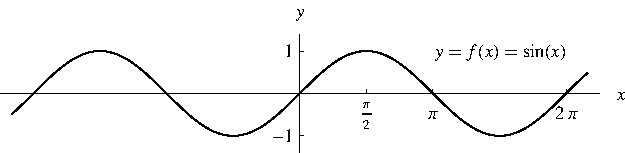
\includegraphics[width=12cm]{derivatives-trig/pictures/03-04-sina.pdf}%
%}%
%\only<handout:0| 2-3>{%
%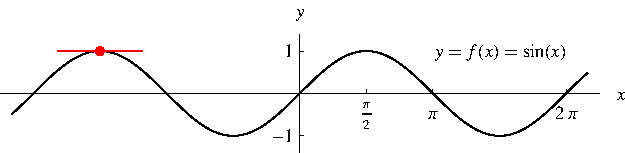
\includegraphics[width=12cm]{derivatives-trig/pictures/03-04-sinb.pdf}%
%}%
%\only<handout:0| 4-5>{%
%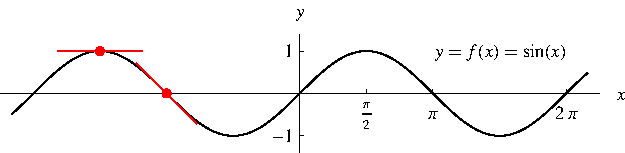
\includegraphics[width=12cm]{derivatives-trig/pictures/03-04-sinc.pdf}%
%}%
%\only<handout:0| 6-7>{%
%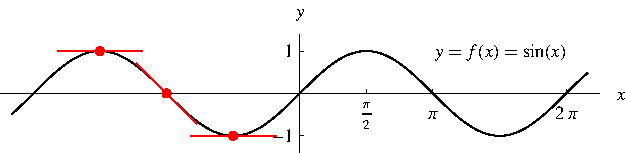
\includegraphics[width=12cm]{derivatives-trig/pictures/03-04-sind.pdf}%
%}%
%\only<handout:0| 8-9>{%
%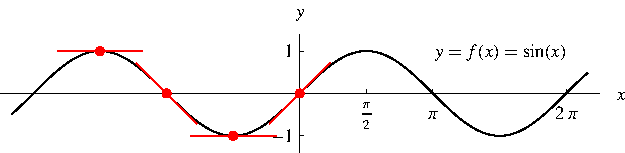
\includegraphics[width=12cm]{derivatives-trig/pictures/03-04-sine.pdf}%
%}%
%\only<handout:0| 10-11>{%
%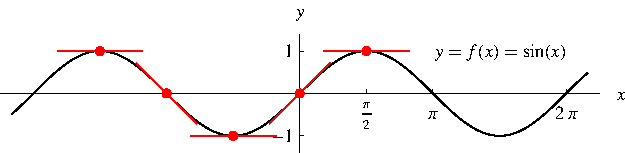
\includegraphics[width=12cm]{derivatives-trig/pictures/03-04-sinf.pdf}%
%}%
%\only<handout:0| 12-13>{%
%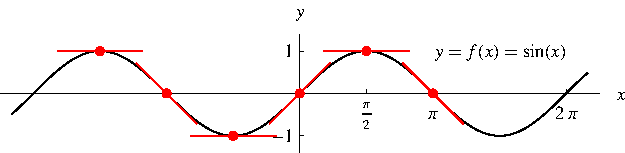
\includegraphics[width=12cm]{derivatives-trig/pictures/03-04-sing.pdf}%
%}%
%\only<14->{%
%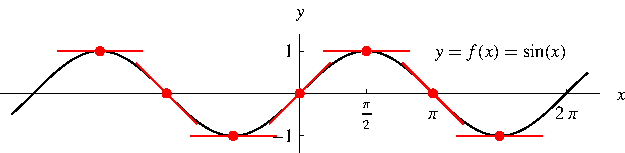
\includegraphics[width=12cm]{derivatives-trig/pictures/03-04-sinh.pdf}%
%}%
%\ \only<handout:0| 1-2>{%
%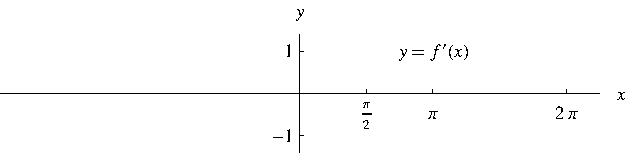
\includegraphics[width=12cm]{derivatives-trig/pictures/03-04-cosa.pdf}%
%}%
%\only<handout:0| 3-4>{%
%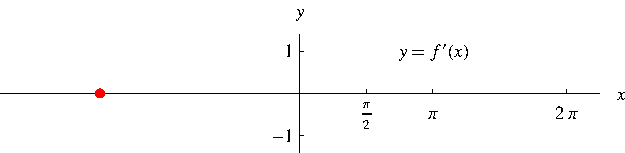
\includegraphics[width=12cm]{derivatives-trig/pictures/03-04-cosb.pdf}%
%}%
%\only<handout:0| 5-6>{%
%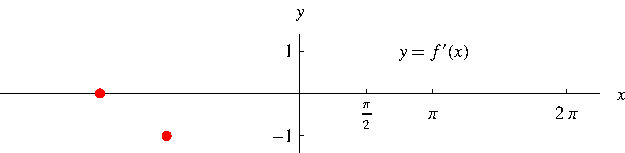
\includegraphics[width=12cm]{derivatives-trig/pictures/03-04-cosc.pdf}%
%}%
%\only<handout:0| 7-8>{%
%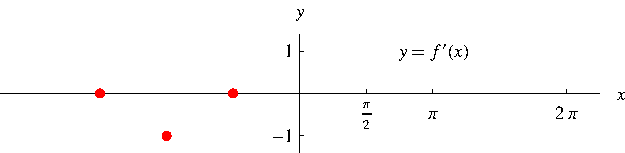
\includegraphics[width=12cm]{derivatives-trig/pictures/03-04-cosd.pdf}%
%}%
%\only<handout:0| 9-10>{%
%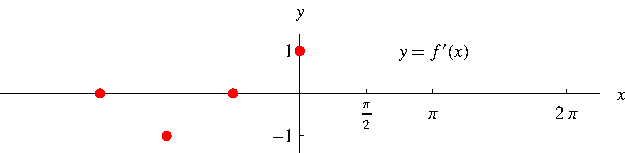
\includegraphics[width=12cm]{derivatives-trig/pictures/03-04-cose.pdf}%
%}%
%\only<handout:0| 11-12>{%
%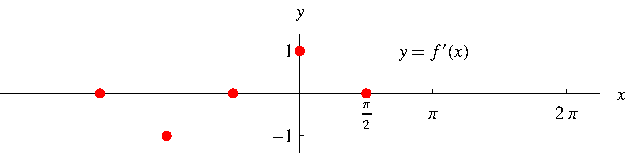
\includegraphics[width=12cm]{derivatives-trig/pictures/03-04-cosf.pdf}%
%}%
%\only<handout:0| 13-14>{%
%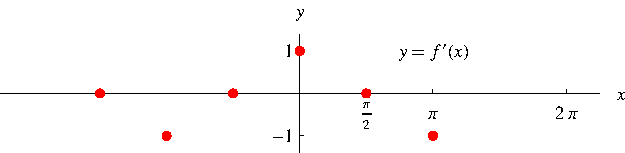
\includegraphics[width=12cm]{derivatives-trig/pictures/03-04-cosg.pdf}%
%}%
%\only<handout:0| 15-16>{%
%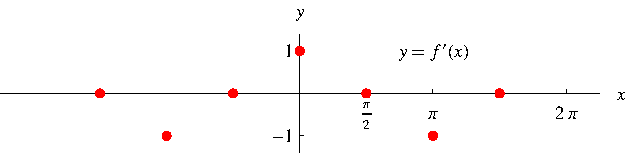
\includegraphics[width=12cm]{derivatives-trig/pictures/03-04-cosh.pdf}%
%}%
%\only<17->{%
%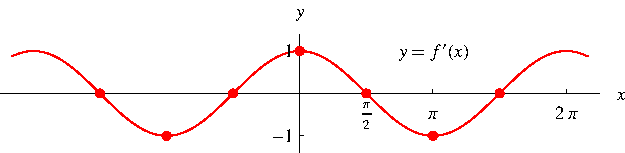
\includegraphics[width=12cm]{derivatives-trig/pictures/03-04-cosi.pdf}%
%}%

What is the derivative of $f(x) = \sin x$?  \uncover<16,17->{It looks like $\cos x$.}
\end{frame}
% end module derivative-sine-graph